%\begin{figure}[H]
%	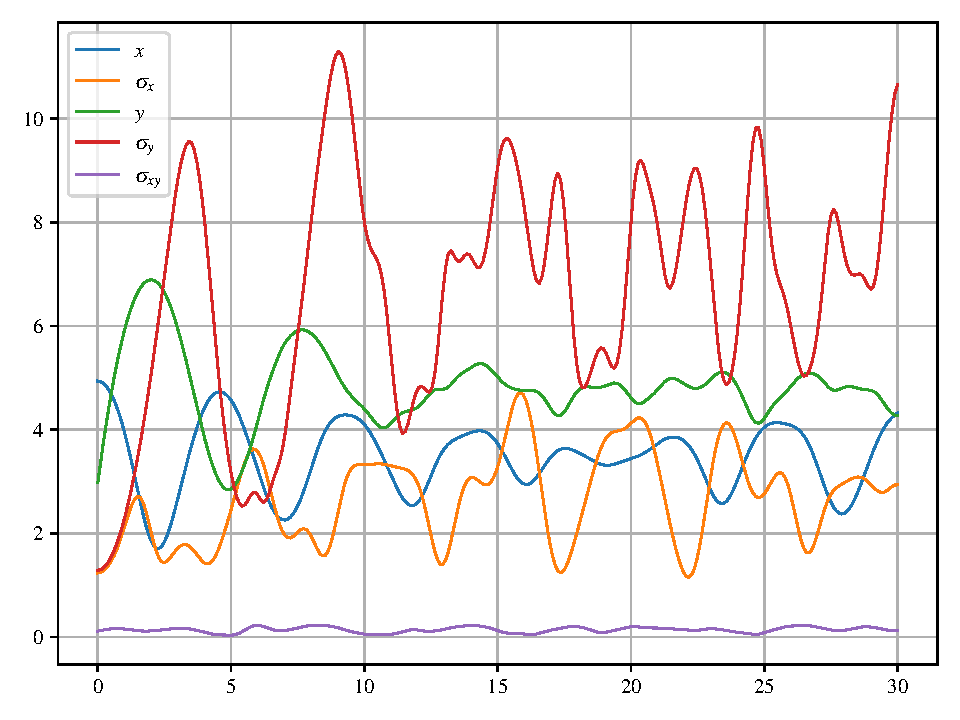
\includegraphics[scale=1]{./figs/expectations.pdf}
%	\caption{Várható értékek és szórások időfejlődése}
%\end{figure}

\begin{lstlisting}[language=Python]
def __init__(self, psi0 = None, F = 1.0, L = 15.0, numPoints = 200, name = "1D: "):
    self.__name = name
    self.__F = F
    self.__L = L
    self.__numPoints = numPoints
    self.__x = np.linspace(0, L, numPoints)
    
    self.__Es = np.zeros((0))
    self.__norms = np.zeros((0))
    self.__cachedBasisFun = np.zeros((0, self.__numPoints), dtype=complex)
    self.__c0s = np.zeros((0))
    
    if psi0 != None:
        self.__unormpsi0 = psi0
        self.__psi0norm = 1 / np.sqrt(np.abs(self.scalarProd(psi0, psi0)))
        n = 0
        while True:
            self.eLevel(n)
            self.waveFunNorm(n)
            self.cacheBasisFun(n)
            self.basisCoeff(n)
            
            eWaveFunSum = np.sum(np.abs(self.__c0s)**2)
            print(self.__name + "Sum of probabilities: " + str(eWaveFunSum))
            if eWaveFunSum > 0.9999:
                break
            n += 1
\end{lstlisting}

\begin{lstlisting}[language=Python]
def charEq(self, E, L = None):
    if L == None:
        L = self.__L
    F3sqrt = np.power(self.__F, 1/3)
    ai1, ai1p, bi1, bi1p = special.airy(-E / F3sqrt ** 2)
    ai1p /= F3sqrt ** 2
    bi1p /= F3sqrt ** 2
    ai2, ai2p, bi2, bi2p = special.airy(F3sqrt * L - E / F3sqrt ** 2)
    ai2p /= F3sqrt ** 2
    bi2p /= F3sqrt ** 2
    f = bi1*ai2 - ai1*bi2
    fp = -(bi1p*ai2 + bi1*ai2p - (ai1p*bi2 + ai1*bi2p))
    return f, fp
\end{lstlisting}

\begin{lstlisting}[language=Python]
def eLevel(self, n):
    '''
    n goes from 0
    '''
    if len(self.__Es) <= n:
        for i in range(len(self.__Es), n+1):
            lstart = 1 / np.power(self.__F, 1/3)
            if self.__L <= lstart:
                llist = np.array([self.__L])
                stepsize = float("nan")
            else:
                stepsize = 0.1
                stepnum = int((self.__L-lstart)//stepsize) + 1
                stepsize = (self.__L-lstart)/stepnum
                llist = np.linspace(lstart, self.__L, stepnum+1)
            Eguess = (np.pi * (i+1) / llist[0]) ** 2
            E = 0
            for l in llist:
                E = (optimize.root_scalar(f=self.charEq, args = (l), x0=Eguess, fprime=True)).root
                Eguess = E * (l/(l+stepsize))**2
            print(self.__name + f"E_{i:d}={E:.2f}")
            self.__Es = np.append(self.__Es, E)
    return
\end{lstlisting}

\begin{lstlisting}[language=Python]
def unormWaveFun(self, x, n):
    '''
    n goes from 0
    '''
    self.eLevel(n)
    E = self.__Es[n]
    F3sqrt = np.power(self.__F, 1/3)
    ai1, ai1p, bi1, bi1p = special.airy(-E / F3sqrt ** 2)
    ai2, ai2p, bi2, bi2p = special.airy(F3sqrt * x - E / F3sqrt ** 2)
    mask = np.array(E / F3sqrt ** 2 - F3sqrt * x > -10).astype(float)
    return (bi1 * ai2 - ai1 * bi2) * mask
\end{lstlisting}

\begin{lstlisting}[language=Python]
def waveFunNorm(self, n):
    '''
    n goes from 0
    '''
    F3sqrt = np.power(self.F, 1/3)
    if len(self.__norms) <= n:
        for i in range(len(self.__norms), n+1):
            self.eLevel(i)
            ai1, ai1p, bi1, bi1p = special.airy(-self.Es[i] / F3sqrt**2)
            ai2, ai2p, bi2, bi2p = special.airy(self.L * F3sqrt - self.Es[i] / F3sqrt**2)
            intsquared = 1 / F3sqrt * (1 / np.pi**2 - (bi1*ai2p - ai1*bi2p * (self.Es[i] - self.L * self.F > -10))**2)
            norm = 1 / np.sqrt(intsquared)
            print(self.__name + f"N_{i:d}={norm:.2f}")
            self.__norms = np.append(self.__norms, norm)
    return
\end{lstlisting}

\begin{lstlisting}[language=Python]
def scalarProd(self, a, b):
    real = integrate.quad(lambda x: np.real(np.conjugate(a(x)) * b(x)), 0, self.__L)[0]
    imag = integrate.quad(lambda x: np.imag(np.conjugate(a(x)) * b(x)), 0, self.__L)[0]
    return real + 1j * imag
\end{lstlisting}

\begin{lstlisting}[language=Python]
def G(self, x, y, E):
    F3sqrt = np.power(self.__F, 1/3)
    ai1, ai1p, bi1, bi1p = special.airy(-E / F3sqrt**2)
    ai2, ai2p, bi2, bi2p = special.airy((self.__F * self.__L - E) / F3sqrt**2)
    ai3, ai3p, bi3, bi3p = special.airy(x * F3sqrt - E / F3sqrt**2)
    ai4, ai4p, bi4, bi4p = special.airy(y * F3sqrt - E / F3sqrt**2)
    c0 = 1 / F3sqrt * np.pi / (ai1/bi1 - ai2/bi2)
    G1 = c0 * (ai4 - ai2/bi2 * bi4) * (ai3 - ai1/bi1 * bi3) * (x < y)
    G2 = c0 * (ai4 - ai1/bi1 * bi4) * (ai3 - ai2/bi2 * bi3) * (1 - (x < y))
    return G1 + G2
\end{lstlisting}

\begin{lstlisting}[language=Python]
def timeEvolution(self, t = 0):
    ret = np.zeros((self.__numPoints), dtype = complex)
    for n in range(len(self.__cachedBasisFun)):
        ret += self.__c0s[n] * np.exp(-1j * self.__Es[n]*t) * self.__cachedBasisFun[n, :]
    return ret
\end{lstlisting}

\begin{lstlisting}[language=Python]
def G(self, x, y, E):
    F3sqrt = np.power(self.__F, 1/3)
    ai1, ai1p, bi1, bi1p = special.airy(-E / F3sqrt**2)
    ai2, ai2p, bi2, bi2p = special.airy((self.__F * self.__L - E) / F3sqrt**2)
    ai3, ai3p, bi3, bi3p = special.airy(x * F3sqrt - E / F3sqrt**2)
    ai4, ai4p, bi4, bi4p = special.airy(y * F3sqrt - E / F3sqrt**2)
    c0 = 1 / F3sqrt * np.pi / (ai1/bi1 - ai2/bi2)
    G1 = c0 * (ai4 - ai2/bi2 * bi4) * (ai3 - ai1/bi1 * bi3) * (x < y)
    G2 = c0 * (ai4 - ai1/bi1 * bi4) * (ai3 - ai2/bi2 * bi3) * (1 - (x < y))
    return G1 + G2
\end{lstlisting}

\begin{lstlisting}[language=Python]
test = d1schroedinger(L=7)

def convergence(E):
    G0 = test.G0(x, y, E)
    VG0 = test.F * x * G0 / N * test.L
    realG = test.G(x, y, E)
    G = G0
    norm0 = dx * np.linalg.norm(G0 @ VG0, ord=2)
    norms = np.array([norm0])
    steps = np.array([0])
    for i in range(20):
        G = G0 + G @ VG0
        norm = dx * np.linalg.norm(G - realG, ord=2)
        norms = np.append(norms, norm)
        steps = np.append(steps, i+1)
        if norm/norm0 + norm0/norm > 5:
            break
    
    popt, pcov = curve_fit(normguess, steps, norms/norms[0])
    return -popt[0]
\end{lstlisting}